\documentclass[convert={imagemagick, density=1024}]{standalone}
\usepackage{amsmath, amsthm, amsfonts,xcolor,pgfplots}
\usepackage{tikz-cd, kotex}
\usetikzlibrary{decorations.markings}
\usepgfplotslibrary{colorbrewer}
\usepackage{../.preamble/quiver}
\usepackage{../.preamble/Operators}
\begin{document}
\nopagecolor

%% Torus_upper (Homology-8.png)
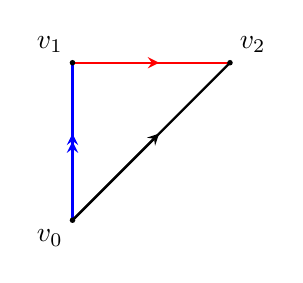
\begin{tikzpicture}[scale=2]
  \draw[-{stealth}, blue, thick] (0,0)--(0,.55); 
  \draw[-{stealth}, blue, thick] (0,0)--(0,.5);
  \draw[blue, thick] (0,0)--(0,1);
  \draw[red, thick] (0,1)--(1,1);
  \draw[red, thick, -{stealth}] (0,1)--(.55,1);
  \draw[thick] (0,0)--(1,1);
  \draw[thick,-{stealth}] (0,0)--(.55,.55);
  \fill (0,0) circle[radius=.5pt] node[below left]{$v_0$};
  \fill (0,1) circle[radius=.5pt] node[above left]{$v_1$};
  \fill (1,1) circle[radius=.5pt] node[above right]{$v_2$};
\end{tikzpicture}



\end{document}

%% Simplices (Homology-1.png)
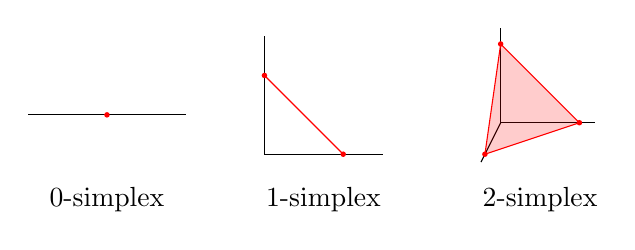
\begin{tikzpicture}
\draw (0, -.7)--(2,-.7);
\fill[red] (1,-.7) circle[radius=1pt];
\draw (1,-1.5) node[below] {$0$-simplex};

\draw (3,-1.2)--(4.5,-1.2);
\draw (3,-1.2)--(3,.3);
\fill[red] (4,-1.2) circle[radius=1pt];
\fill[red] (3,-.2) circle[radius=1pt];
\draw[red] (3,-.2)--(4,-1.2);
\draw (3.75,-1.5) node[below] {$1$-simplex};

\draw (6,-.8)--(7.2,-.8);
\draw (6,-.8)--(6,.4);
\draw (6,-.8)--(5.75,-1.3);
\fill[red] (7,-.8) circle[radius=1pt];
\fill[red] (6,.2) circle[radius=1pt];
\fill[red] (5.8,-1.2) circle[radius=1pt];
\draw[red, fill=red, fill opacity=.2] (6,.2)--(7,-.8)--(5.8,-1.2)--cycle;
\draw (6.5,-1.5) node[below] {$2$-simplex};
\end{tikzpicture}

%% Torus_2D (Homology-2.png)
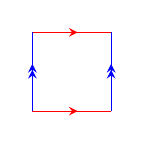
\begin{tikzpicture}
  \fill[white] (-.06,-.06) rectangle (1.06,1.06);
  \draw[-{stealth}, red] (0,0) -- (.575,0);
  \draw[red] (0,0) -- (1,0);
  \draw[-{stealth}, red] (0,1) -- (.575,1);
  \draw[red] (0,1) -- (1,1);
  \draw[-{stealth}, blue] (0,0) -- (0,.6);
  \draw[-{stealth}, blue] (0,0) -- (0,.525);
  \draw[blue] (0,0) -- (0,1);
  \draw[-{stealth}, blue] (1,0) -- (1,.6);
  \draw[-{stealth}, blue] (1,0) -- (1,.525);
  \draw[blue] (1,1) -- (1,0);
\end{tikzpicture}

%% Torus_3D (Homology-3.png)
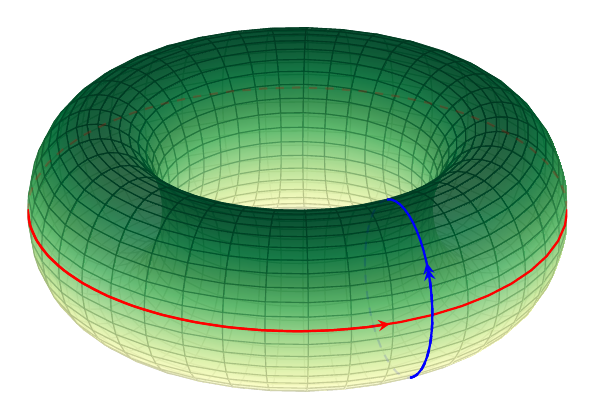
\begin{tikzpicture}
  \begin{axis}[view={180}{50}, axis lines=none, colormap/YlGn]
    % Draw the torus surface
    \addplot3[
      surf,
      shader=faceted interp, 
      samples=40,
      domain=0:360,
      y domain=0:360,
      z buffer=sort,
      opacity=.8
    ]
    (
      { (3 + cos(x)) * cos(y) },
      { (3 + cos(x)) * sin(y) },
      { sin(x) }
    );
    \addplot3+ [red, thick,
      domain=0:180,
        samples y=0,
        mark=none
    ]
    (
      { 4 * cos(x) },
      { 4 * sin(x) },
      { 0 }
    );
    \addplot3+ [red, thick,
      domain=0:110,
        samples y=0,
        mark=none,
        -{stealth}
    ]
    (
      { 4 * cos(x) },
      { 4 * sin(x) },
      { 0 }
    );
    \addplot3+ [red, thick, opacity=.2, dashed,
      domain=180:360,
        samples y=0,
        mark=none
    ]
    (
      { 4 * cos(x) },
      { 4 * sin(x) },
      { 0 }
    );
    \addplot3+ [blue, thick,
      domain=-70:110,
        samples y=0,
        mark=none
    ]
    (
      { (3 + cos(x)) * cos(120) },
      { (3 + cos(x)) * sin(120) },
      { sin(x) }
    );
    \addplot3+ [blue, thick,
      domain=-70:30,
        samples y=0,
        mark=none,
        -{stealth}
    ]
    (
      { (3 + cos(x)) * cos(120) },
      { (3 + cos(x)) * sin(120) },
      { sin(x) }
    );
    \addplot3+ [blue, thick,
      domain=-70:34,
        samples y=0,
        mark=none,
        -{stealth}
    ]
    (
      { (3 + cos(x)) * cos(120) },
      { (3 + cos(x)) * sin(120) },
      { sin(x) }
    );
    \addplot3+ [blue, thick, opacity=.1, dashed,
      domain=110:290,
        samples y=0,
        mark=none
    ]
    (
      { (3 + cos(x)) * cos(120) },
      { (3 + cos(x)) * sin(120) },
      { sin(x) }
    );
  \end{axis}
\end{tikzpicture}

%% Mobius_strip_2D (Homology-4.png)
\begin{tikzpicture}
  \fill[white] (-.06,-.06) rectangle (1.06,1.06);
  \draw[-{stealth}, red] (0,0) -- (.575,0);
  \draw[red] (0,0) -- (1,0);
  \draw[-{stealth}, red] (1,1) -- (.425,1);
  \draw[red] (0,1) -- (1,1);
  \draw[green!50!black] (0,0) -- (0,1);
  \draw[green!50!black] (1,1) -- (1,0);
\end{tikzpicture}

%% Mobius_strip_3D (Homology-5.png)
 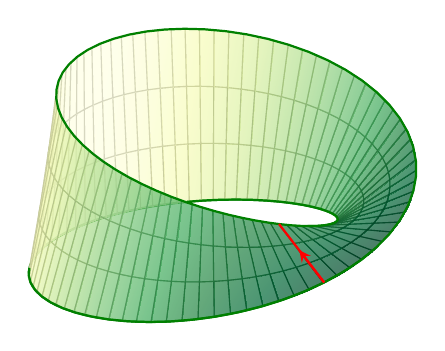
\begin{tikzpicture}
    \begin{axis}[
    hide axis,
    view = {40}{40},
    colormap/YlGn
    ]
    \addplot3 [color=green!50!black,thick,    
    domain     = 360:720,samples y=0, samples=80,
    ] (
    {(1+0.5*0.5*cos(x/2)))*cos(x)},
    {(1+0.5*0.5*cos(x/2)))*sin(x)},
    {0.5*0.5*sin(x/2)}
    );
    \addplot3 [
    surf,
    shader     = faceted interp,opacity = 0.7,
    %shader = interp,
    point meta = x,
    samples    = 80,
    samples y  = 4,
    z buffer   = sort,
    domain     = 0:360,
    y domain   =-0.5:0.5
    ] (
    {(1+0.5*y*cos(x/2)))*cos(x)},
    {(1+0.5*y*cos(x/2)))*sin(x)},
    {0.5*y*sin(x/2)}
    );
    \addplot3 [color=green!50!black,thick,    
    domain     = -140:497.5,samples y=0,samples=100,
    ] (
    {(1+0.5*0.5*cos(x/2)))*cos(x)},
    {(1+0.5*0.5*cos(x/2)))*sin(x)},
    {0.5*0.5*sin(x/2)}
    );
    \addplot3 [color=red,thick,    
    domain     = -.5:.5,samples y=0,samples=100,
    ] (
    {(1+0.5*x*cos(171)))*cos(342)},
    {(1+0.5*x*cos(171)))*sin(342)},
    {0.5*x*sin(171)}
    );
    \addplot3 [color=red,thick,    
    domain     = -.5:.05,samples y=0,samples=100,-{stealth}
    ] (
    {(1+0.5*x*cos(171)))*cos(342)},
    {(1+0.5*x*cos(171)))*sin(342)},
    {0.5*x*sin(171)}
    );
    \end{axis}
 \end{tikzpicture}

 %% Torus (Homology-6.png)
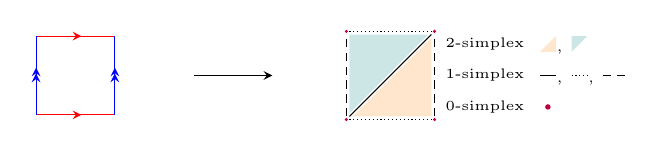
\begin{tikzpicture}
  \draw[white] (-.1,-.1) rectangle (7.5,1.1);
  \draw[-{stealth}, red] (0,0) -- (.575,0);
  \draw[red] (0,0) -- (1,0);
  \draw[-{stealth}, red] (0,1) -- (.575,1);
  \draw[red] (0,1) -- (1,1);
  \draw[-{stealth}, blue] (0,0) -- (0,.6);
  \draw[-{stealth}, blue] (0,0) -- (0,.525);
  \draw[blue] (0,0) -- (0,1);
  \draw[-{stealth}, blue] (1,0) -- (1,.6);
  \draw[-{stealth}, blue] (1,0) -- (1,.525);
  \draw[blue] (1,1) -- (1,0);

  \draw[-{stealth}] (2,.5) -- (3,.5);
  \fill[orange, opacity=.2] (4.02,-.02) -- (5.02,-.02) -- (5.02,0.98) -- cycle;
  \fill[teal, opacity=.2] (3.98,0.02) -- (3.98,1.02) -- (4.98,1.02) -- cycle;
  \draw (3.98,-.02) -- (5.02,1.02);
  \draw[densely dashed] (3.94,-.02) -- (3.94,1.02);
  \draw[densely dotted] (3.98,1.06) -- (5.02,1.06);
  \draw[densely dashed] (5.06,-.02) -- (5.06,1.02);
  \draw[densely dotted] (3.98,-.06) -- (5.02,-.06);
  \fill[purple] (3.94,1.06) circle[radius=.6pt];
  \fill[purple] (5.06,1.06) circle[radius=.6pt];
  \fill[purple] (3.94,-.06) circle[radius=.6pt];
  \fill[purple] (5.06,-.06) circle[radius=.6pt];
  \draw (5.7,.9) node{\tiny $2$-simplex};
  \fill[orange, opacity=.2] (6.4,.8)--(6.6,.8)--(6.6,1)--cycle;
  \draw (6.65,.8) node{\tiny,};
  \fill[teal, opacity=.2] (6.8,.8)--(6.8,1)--(7,1)--cycle;
  \draw (5.7,.5) node{\tiny $1$-simplex};
  \draw (6.4,.5)--(6.6,.5);
  \draw (6.65,.4) node{\tiny,};
  \draw[densely dotted] (6.8,.5)--(7,.5);
  \draw (7.05,.4) node{\tiny,};
  \draw[densely dashed] (7.2,.5)--(7.5,.5);
  \draw (5.7,.1) node{\tiny $0$-simplex};
  \fill[purple] (6.5,.1) circle[radius=1pt];
\end{tikzpicture}

%%Finer_torus (Homology-7.png)
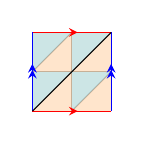
\begin{tikzpicture}
  \fill[white] (-.06,-.06) rectangle (1.06,1.06);
  \draw[gray!50] (.5,0)--(.5,1);
  \draw[gray!50] (0,.5)--(1,.5);
  \draw[gray!50] (0,.5)--(.5,1);
  \draw[gray!50] (.5,0)--(1,.5);
  \fill[teal, opacity=.2] (0,0) -- (.5,.5) -- (0,.5) -- cycle;
  \fill[teal, opacity=.2] (0,.5) -- (.5,1) -- (0,1) -- cycle;
  \fill[teal, opacity=.2] (.5,.5) -- (1,1) -- (.5,1) -- cycle;
  \fill[teal, opacity=.2] (.5,0) -- (1,.5) -- (.5,.5) -- cycle;
  \fill[orange, opacity=.2] (0,0) -- (.5,.5) -- (.5,0) -- cycle;
  \fill[orange, opacity=.2] (0,.5) -- (.5,1) -- (.5,.5) -- cycle;
  \fill[orange, opacity=.2] (.5,.5) -- (1,1) -- (1,.5) -- cycle;
  \fill[orange, opacity=.2] (.5,0) --(1,.5) -- (1,0) -- cycle;
  \draw[-{stealth}, red] (0,0) -- (.575,0);
  \draw[red] (0,0) -- (1,0);
  \draw[-{stealth}, red] (0,1) -- (.575,1);
  \draw[red] (0,1) -- (1,1);
  \draw[-{stealth}, blue] (0,0) -- (0,.6);
  \draw[-{stealth}, blue] (0,0) -- (0,.525);
  \draw[blue] (0,0) -- (0,1);
  \draw[-{stealth}, blue] (1,0) -- (1,.6);
  \draw[-{stealth}, blue] (1,0) -- (1,.525);
  \draw[blue] (1,1) -- (1,0);
  \draw (0,0) -- (1,1);
\end{tikzpicture}

%% Torus_upper (Homology-8.png)
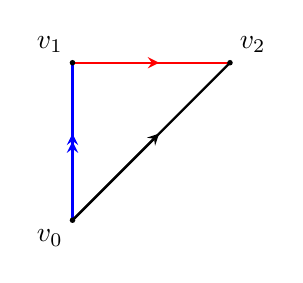
\begin{tikzpicture}[scale=2]
  \draw[-{stealth}, blue, thick] (0,0)--(0,.55); 
  \draw[-{stealth}, blue, thick] (0,0)--(0,.5);
  \draw[blue, thick] (0,0)--(0,1);
  \draw[red, thick] (0,1)--(1,1);
  \draw[red, thick, -{stealth}] (0,1)--(.55,1);
  \draw[thick] (0,0)--(1,1);
  \draw[thick,-{stealth}] (0,0)--(.55,.55);
  \fill (0,0) circle[radius=.5pt] node[below left]{$v_0$};
  \fill (0,1) circle[radius=.5pt] node[above left]{$v_1$};
  \fill (1,1) circle[radius=.5pt] node[above right]{$v_2$};
\end{tikzpicture}

%% Torus_lower (Homology-9.png)
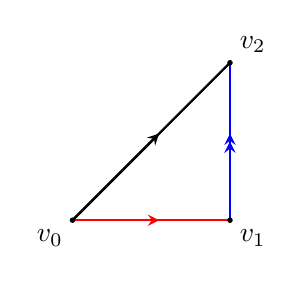
\begin{tikzpicture}[scale=2]
  \draw[-{stealth}, blue, thick] (1,0)--(1,.55); 
  \draw[-{stealth}, blue, thick] (1,0)--(1,.5);
  \draw[blue, thick] (1,0)--(1,1);
  \draw[red, thick] (0,0)--(1,0);
  \draw[red, thick, -{stealth}] (0,0)--(.55,0);
  \draw[thick] (0,0)--(1,1);
  \draw[thick,-{stealth}] (0,0)--(.55,.55);
  \fill (0,0) circle[radius=.5pt] node[below left]{$v_0$};
  \fill (1,0) circle[radius=.5pt] node[below right]{$v_1$};
  \fill (1,1) circle[radius=.5pt] node[above right]{$v_2$};
\end{tikzpicture}